\section{Tutorial: Erstellung einer verteilten TensorFlow Umgebung}
Nachdem im vorherigen Kapitel das Konzept einer verteilten TensorFlow Umgebung erläutert wurde, wollen wir Schritt für Schritt eine solche Umgebung einrichten.

\subsection{Vorbereitung der Instanzen}
Als erstes müssen wir vier Instanzen aufsetzen. Wenn möglich sollte jede Instanz die gleichen Ressourcen zur Verfügung haben. In meinem Fall habe ich vier virtuelle Maschinen in der StudiCloud der Hochschule Furtwangen erstellt. Jede virtuelle Maschine hat eine virtuelle \ac{cpu}, 1GB RAM und 10GB Festplattenspeicher zur Verfügung. Auf den virtuellen Maschinen wurde Ubuntu Server 16.04 installiert. Um die Kommunikation unter den virtuellen Maschinen zu vereinfachen, setzen wir wie in Abbildung \ref{fig:hostkonfiguration} für jede virtuelle Maschine einen Hostname und die anderen virtuellen Maschinen als Hosts. 

\begin{figure}[h!]
	\centering
	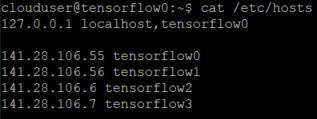
\includegraphics[width=0.9\linewidth]{Pictures/HostKonfiguration}
	\caption[Hosts Konfiguration]{Exemplarische Hosts Konfiguration}
	\label{fig:hostkonfiguration}
\end{figure}

Im Idealfall sollten Instanzen mit wesentlich mehr \ac{cpu} Leistung und einer zusätzlichen Grafikkarte eingesetzt werden, da nur so eine optimale Performance möglich ist. Im Rahmen dieser Arbeit standen mir diese Mittel nicht zur Verfügung.

\subsection{Installation von TensorFlow}
Nun müssen wir auf den virtuellen Maschinen Python und TensorFlow installieren. Python benötigen wir zum Entwickeln unserer Beispielanwendung und wir nutzen Python's Paketmanager pip zur Installation von TensorFlow. Dazu müssen folgende Befehle auf den virtuellen Maschinen ausgeführt werden.
\begin{itemize}
	\item Installation von Python zur Entwicklung:\newline
			\texttt{sudo apt-get install python3-dev}
	\item Installation von Python's Paketmanager pip\newline
			\texttt{sudo apt-get install python3-pip}
	\item Installation von TensorFlow via pip\newline
			\texttt{pip3 install tensorflow}
\end{itemize}

\subsection{Entwicklung einer Anwendung}
Die virtuellen Maschinen mit einer Python- und TensorFlow Installation sind jetzt einsatzbereit. Jetzt wollen wir eine einfache TensorFlow Anwendung erstellen, die eine virtuelle Maschine als Parameterserver und zwei virtuelle Maschinen als Arbeiter nutzt. Wir entwickeln die Anwendung lokal auf unserem Computer und verteilen sie danach auf die virtuelle Maschinen. Dazu erstellen wir die Datei \textit{"train.py"} und öffnen sie in einer Entwicklungsumgebung unser Wahl (in meinem Fall Visual Studio Code). 

\vspace{2mm}
\subsubsection{Erstellung eines Clusters}
Als erstes müssen wir ein Cluster aus Arbeiter und Parameterserver Instanzen definieren. Diese werden bei Anwendungsstart in den Argumenten "\textit{--worker\_hosts}" und "\textit{--ps\_hosts}" übergeben. Dies bietet den Vorteil, dass wir die gleiche Anwendung für Arbeiter bzw. Parameterserver verwenden können.

\begin{itemize}
	\item Parsen der Argumenten: \newline
		\texttt{ps\_hosts = FLAGS.ps\_hosts.split(",")} \newline
		\texttt{ps\_hosts = FLAGS.ps\_hosts.split(",")}
	\item Erstellung des Clusters mit den Arbeitern und Parameterservern anhand der Parameter: \newline
			\texttt{cluster = tf.train.ClusterSpec({"ps": ps\_hosts, "worker": worker\_hosts})}
\end{itemize}

\vspace{2mm}
\subsubsection{Starten der Instanz}
Nachdem wir ein Cluster erstellt haben, müssen wir die jeweilige Instanz starten, dazu nutzen wir die Argumente "\textit{--job\_name}" und "\textit{--task\_index}".
\begin{itemize}
	\item Starten der Instanz: \newline
		\texttt{server = tf.train.Server(cluster,
				job\_name=FLAGS.job\_name,	
				task\_index=FLAGS.task\_index)}
\end{itemize}

\vspace{2mm}
\subsubsection{Parameterserver}
Als nächstes ist abzuklären, ob die aktuelle Instanz als Arbeiter oder Parameterserver dienen soll. Wenn die Instanz als Parameterserver dient, soll sie keine Berechnung durchführen, sondern warten bis ein Arbeiter Attribute anfordert oder aktualisieren will.
\begin{itemize}
	\item Initialisierung einer Instanz als Parameterserver: \newline
		\texttt{if FLAGS.job\_name == 'ps': 
			server.join()}
\end{itemize}

\vspace{2mm}
\subsubsection{Arbeiter}
Wenn eine Instanz kein Parameterserver ist, ist sie automatisch ein Arbeiter und führt Berechnungen durch. Die Arbeiter führen ihre Berechnungen synchron durch und warten deshalb nach jeder Iteration, bis jeder Arbeiter die Variablen auf dem Parameterserver synchronisiert hat. Anschließend verteilt der Parameterserver wieder die aktualisierten Variablen an die Arbeiter. Wir wollen dabei nicht genauer auf die Berechnungen eingehen und nutzen daher einen Beispielcode eines Tutorials von TensorFlow und schauen uns an, wie eine Berechnung auf einem Arbeiter durchgeführt wird:

\begin{itemize}
	\item Zuweisung einer Berechnung zu einem Arbeiter: \newline
		\texttt{with tf.device(tf.train \newline
			\hspace*{5mm} .replica\_device\_setter(
			\hspace*{5mm} worker\_device="/job:worker/task:\%d",\newline
			\hspace*{5mm} \% FLAGS.task\_index, cluster=cluster)):}
	\item Parsen des Arguments "is\_chief", welches angibt, ob ein Arbeiter als Master fungiert: \newline
		\texttt{is\_chief = (FLAGS.task\_index == 0)}
	\item Starten einer neuen Session auf einem Arbeiter: \newline
		\texttt{sess = tf.train.MonitoredTrainingSession(
			master=server.target,
			is\_chief=is\_chief)}
	\item Starten einer Berechnung in der Session: \newline
		\texttt{sess.run(task)}
	\item Beenden einer Session, sobald die Berechnung beendet wurde: \newline
		\texttt{sess.close()}
\end{itemize}

Nun haben wir alle wichtigen Konfigurationen für unsere verteilte TensorFlow Umgebung vorgenommen. Der komplette Quellcode der Beispielanwendung kann unter "https://github.com/MichZipp/Exploring-Distributed-Tensorflow/Code" gefunden werden. 

\subsection{Starten einer Anwendung}
Jetzt müssen wir die Anwendung noch starten, dazu müssen wir zuerst unsere \textit{"train.py"} mit dem \ac{ftp} auf unsere Instanzen kopieren. Als nächstes müssen wir die Anwendung auf jeder Instanz mit den richtigen Argumenten starten. Um diesen Prozess zu vereinfachen, schreiben wir uns ein kleines Bash-Skript, das wir dann nur auf dem Master Arbeiter starten müssen:

\begin{itemize}
	\item Bash-Script \textit{"run.sh"} für ein Cluster aus zwei Arbeitern und einem Parameterserver: \newline
		\texttt{\#!/bin/bash \newline
			ssh clouduser@tensorflow2 \newline
			\hspace*{5mm} 'python3 ~/Tensorflow/trainer.py \newline
			\hspace*{5mm} --ps\_hosts="tensorflow2:2222" \newline
			\hspace*{5mm} --worker\_hosts="tensorflow0:2222, \newline 
			\hspace*{10mm} tensorflow1:2222" \newline
			\hspace*{5mm} --job\_name="ps" --task\_index=0' \newline
			ssh clouduser@tensorflow1 \newline
			\hspace*{5mm} 'python3 ~/Tensorflow/trainer.py \newline
			\hspace*{5mm} --ps\_hosts="tensorflow2:2222" \newline
			\hspace*{5mm} --worker\_hosts="tensorflow0:2222, \newline
			\hspace*{10mm} tensorflow1:2222" \newline
			\hspace*{5mm} --job\_name="worker" --task\_index=1' \newline
			python3 ~/Tensorflow/trainer.py \newline
			\hspace*{5mm} --ps\_hosts="tensorflow2:2222" \newline
			\hspace*{5mm} --worker\_hosts="tensorflow0:2222, \newline
			\hspace*{10mm} tensorflow1:2222" \newline
			\hspace*{5mm} --job\_name="worker" --task\_index=0}
	\item Ausführen des Bash-Skripts: \newline
		\texttt{bash run.sh}
\end{itemize}

\vspace{2mm}
Um die Cluster-Zusammenstellungen zu verändern, muss nur das Bash-Skript angepasst werden. Bei vier Instanzen können folgende Cluster-Zusammenstellungen verwendet werden:

\begin{itemize}
	\item 1 Arbeiter, 1 Parameterserver
	\item 2 Arbeiter, 1 Parameterserver
	\item 3 Arbeiter, 1 Parameterserver
	\item 1 Arbeiter, 2 Parameterserver
	\item 1 Arbeiter, 3 Parameterserver
	\item 2 Arbeiter, 2 Parameterserver
\end{itemize}

Wie dieses Tutorial zeigt, sind nicht viele Schritte notwendig, um eine verteilte TensorFlow Umgebung einzurichten. 




